% The four operator formats of the tangent, from matrix-free application to the assembled matrix:
% what the set-up builds once per Newton step and what each application does; below, the two steps
% of measures that shrink the stored formats (exact reductions, then encodings).
\documentclass[border=2pt]{standalone}
% Shared preamble of the format diagrams: colours of the paper's figures (paper_figures.py) and
% the drawing styles.  Each diagram is a standalone document built to a PDF of the text width.
\usepackage{amsmath,amssymb}
\usepackage{tikz}
\usetikzlibrary{arrows.meta,calc,decorations.pathreplacing,patterns,positioning}

\definecolor{cindex}{HTML}{BDBDBD}  % column indices, offsets, row pointers
\definecolor{cvalue}{HTML}{6E6E6E}  % floating-point values (BSR)
\definecolor{cpoint}{HTML}{1B9E77}  % quadrature-point store
\definecolor{celem}{HTML}{1F78B4}   % element matrix
\definecolor{cqbsr}{HTML}{A6761D}   % quantized BSR
\definecolor{cscale}{HTML}{E6AB02}  % scales
\definecolor{cmean}{HTML}{7570B3}   % f32 element mean

\tikzset{
  >={Stealth[length=4pt]},
  grid/.style={draw=black!45, line width=0.25pt},
  frame/.style={draw=black!70, line width=0.5pt},
  title/.style={font=\small\bfseries, anchor=west, inner sep=0pt},
  lab/.style={font=\footnotesize, inner sep=1pt},
  note/.style={font=\scriptsize, text=black!75, inner sep=1pt, execute at begin node={\hyphenpenalty=10000\exhyphenpenalty=10000}},
  num/.style={font=\tiny, inner sep=0pt},
  brace/.style={decorate, decoration={brace, amplitude=3pt, raise=1pt}, line width=0.4pt},
  arr/.style={->, line width=0.5pt, black!70},
  pad/.style={pattern=north east lines, pattern color=black!30},
}

% \cell{x}{y}{w}{h}{fill}: a filled rectangle with a thin outline, lower-left corner at (x,y).
\newcommand{\cell}[5]{\filldraw[fill=#5, grid] (#1,#2) rectangle ++(#3,#4);}
% \blk{x}{y}{s}{fill}: a 3x3 block of side s with its 3x3 entry grid.
\newcommand{\blk}[4]{%
  \filldraw[fill=#4, grid] (#1,#2) rectangle ++(#3,#3);
  \draw[draw=white, line width=0.25pt] (#1,#2) ++(#3/3,0) -- ++(0,#3) ++(#3/3,0) -- ++(0,-#3);
  \draw[draw=white, line width=0.25pt] (#1,#2) ++(0,#3/3) -- ++(#3,0) ++(0,#3/3) -- ++(-#3,0);
  \draw[grid] (#1,#2) rectangle ++(#3,#3);}
% \vthree{x}{y}{fill}: a 3-vector (one node's components) as three small cells, left end at (x,y).
\newcommand{\vthree}[3]{\foreach \k in {0,1,2} \filldraw[fill=#3, grid] (#1+\k*0.14,#2) rectangle ++(0.14,0.14);}
% \op{x}{y}{symbol}: an operation in a small circle.
\newcommand{\op}[3]{\node[circle, draw=black!70, line width=0.4pt, inner sep=0.5pt, minimum size=9pt, font=\tiny] at (#1,#2) {#3};}

\begin{document}
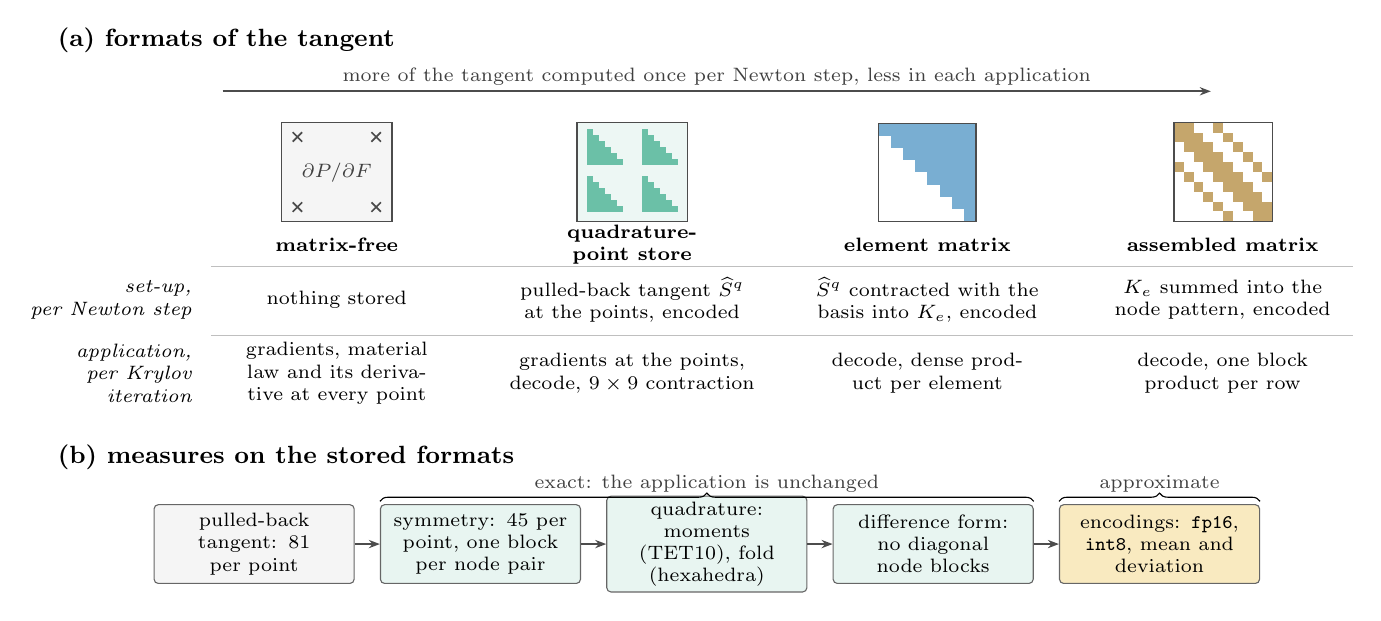
\begin{tikzpicture}
  \tikzset{
    col/.style={font=\scriptsize, align=center, text width=3.15cm, inner sep=1pt},
    rowlab/.style={font=\scriptsize\itshape, anchor=east, align=right, inner sep=1pt},
    mstep/.style={draw=black!60, line width=0.4pt, rounded corners=1.5pt, font=\scriptsize, align=center,
                 text width=2.4cm, minimum height=1.0cm, inner sep=2pt},
  }
  \def\dx{3.75}
  % ---------------------------------------------------------------- (a) the formats
  \node[title] at (-1.9, 4.85) {(a) formats of the tangent};
  \draw[arr, line width=0.6pt] (0.2,4.2) -- (3*\dx+1.5,4.2)
    node[midway, above=1pt, note] {more of the tangent computed once per Newton step, less in each application};

  % matrix-free: an element with its points, the law evaluated at each
  \begin{scope}[shift={(0,2.55)}]
    \draw[frame, fill=black!4] (0.95,0) rectangle (2.35,1.25);
    \foreach \x/\y in {1.15/0.18, 2.15/0.18, 1.15/1.07, 2.15/1.07}
      \draw[black!70, line width=0.6pt] (\x-0.06,\y-0.06) -- (\x+0.06,\y+0.06) (\x-0.06,\y+0.06) -- (\x+0.06,\y-0.06);
    \node[note] at (1.65,0.62) {$\partial P/\partial F$};
  \end{scope}
  % quadrature-point store: the stored tangent at each point
  \begin{scope}[shift={(\dx,2.55)}]
    \draw[frame, fill=cpoint!8] (0.95,0) rectangle (2.35,1.25);
    \def\t{0.075}
    \foreach \x/\y in {1.08/0.12, 1.78/0.12, 1.08/0.72, 1.78/0.72}
      \foreach \r in {0,...,5} \foreach \c in {0,...,\r}
        \fill[cpoint!65] (\x+\c*\t, \y+0.45-\r*\t) rectangle ++(\t,-\t);
  \end{scope}
  % element matrix: the dense element block
  \begin{scope}[shift={(2*\dx,2.55)}]
    \def\s{0.155}
    \foreach \p in {0,...,7} \foreach \q in {0,...,7} {
      \pgfmathparse{\q>=\p ? 1 : 0}
      \ifnum\pgfmathresult=1 \fill[celem!60] (1.03+\q*\s, 1.24-\p*\s) rectangle ++(\s,-\s); \fi
    }
    \draw[frame] (1.03,0) rectangle ++(8*\s,8*\s);
  \end{scope}
  % assembled matrix: a sparse block pattern
  \begin{scope}[shift={(3*\dx,2.55)}]
    \def\s{0.125}
    \foreach \i in {0,...,9} \foreach \j in {0,...,9} {
      \pgfmathparse{abs(\i-\j)<=1 || abs(\i-\j)==4 ? 1 : 0}
      \ifnum\pgfmathresult=1 \fill[cqbsr!65] (1.03+\j*\s, 1.25-\i*\s) rectangle ++(\s,-\s); \fi
    }
    \draw[frame] (1.03,0) rectangle ++(10*\s,10*\s);
  \end{scope}

  \foreach \name [count=\c from 0] in {matrix-free, quadrature-point store, element matrix, assembled matrix}
    \node[col, font=\scriptsize\bfseries] at ({\c*\dx+1.65}, 2.25) {\name};
  \node[rowlab] at (-0.15, 1.55) {set-up,\\per Newton step};
  \node[rowlab] at (-0.15, 0.62) {application,\\per Krylov\\iteration};
  \foreach \txt [count=\c from 0] in {
      {nothing stored},
      {pulled-back tangent $\widehat S^q$ at the points, encoded},
      {$\widehat S^q$ contracted with the basis into $K_e$, encoded},
      {$K_e$ summed into the node pattern, encoded}}
    \node[col] at ({\c*\dx+1.65}, 1.55) {\txt};
  \foreach \txt [count=\c from 0] in {
      {gradients, material law and its derivative at every point},
      {gradients at the points, decode, $9\times9$ contraction},
      {decode, dense product per element},
      {decode, one block product per row}}
    \node[col] at ({\c*\dx+1.65}, 0.62) {\txt};
  \draw[grid, draw=black!25] (0.05,1.1) -- (3*\dx+3.3,1.1);
  \draw[grid, draw=black!25] (0.05,1.98) -- (3*\dx+3.3,1.98);

  % ---------------------------------------------------------------- (b) the measures
  \node[title] at (-1.9, -0.45) {(b) measures on the stored formats};
  \begin{scope}[shift={(0,-1.55)}]
    \node[mstep, fill=black!4] (s0) at (0.6,0) {pulled-back\\tangent: $81$\\per point};
    \node[mstep, fill=cpoint!10, right=0.32cm of s0] (s1) {symmetry: $45$ per\\point, one block\\per node pair};
    \node[mstep, fill=cpoint!10, right=0.32cm of s1] (s2) {quadrature: moments\\(TET10), fold\\(hexahedra)};
    \node[mstep, fill=cpoint!10, right=0.32cm of s2] (s3) {difference form:\\no diagonal\\node blocks};
    \node[mstep, fill=cscale!25, right=0.32cm of s3] (s4) {encodings: \texttt{fp16},\\\texttt{int8}, mean and\\deviation};
    \foreach \a/\b in {s0/s1, s1/s2, s2/s3, s3/s4} \draw[arr] (\a) -- (\b);
    \draw[brace] (s1.north west) -- (s3.north east) node[midway, above=3pt, note] {exact: the application is unchanged};
    \draw[brace] (s4.north west) -- (s4.north east) node[midway, above=3pt, note] {approximate};
  \end{scope}
\end{tikzpicture}
\end{document}
